\section{Rolando}

\subsection{Diagrama GANTT}

El siguiente diagrama fue generado con los siguientes parametros:

\begin{enumerate}
	\item lote\_tsk: 2.tsk
	\item num\_cores: 1
	\item switch\_cost: 4
	\item sched\_class: SchedFCFS
\end{enumerate}

\begin{figure}[h]
    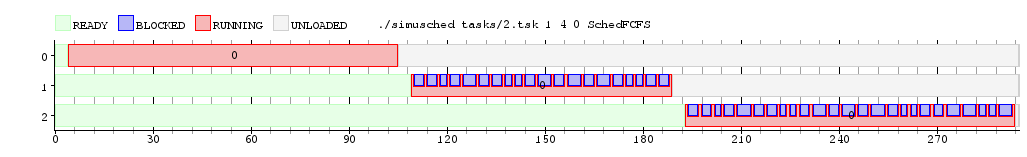
\includegraphics[width=\linewidth]{images/2_1nucleo.png}
    \label{fig:Task Consola}
    \caption{Rolando con 1 núcleo}
\end{figure}

En la figura 2 se presenta el diagrama de Gantt del \textit{lote2} bajo el algortimo del scheduler FCFS. Este lote simula la situaci\'on de \textit{Rolando}, para la que se requiere ejecutar 3 tareas. Las tres tendr\'an un \textit{release time} nulo, de modo que cada tarea s\'olo deber\'a esperar al costo de cambio de contexto para entrar en estado \textit{runing}. La primera, que es del tipo TaskCPU y con su parametro igual a 100, tras esperar 4 ciclos de reloj (por el \textit{switch\_cost}), como su parametro indica, hace uso del CPU durante 100 ciclos de rejoj, y uno extra por la llamada a \textit{exit()}. Tras finalizar la anterior, y despu\'es de otros 4 ciclos por el cambio de contexto, pasa al estado \textit{runing} la segunda tarea, esta vez de tipo TaskConsola y con el vector \textit{$<$20, 2, 4$>$} como parametro. Esta efectua 20 llamadas bloqueantes, que demoran entre 2 a 4 ciclos, haciendo uso de 20 llamadas consecutivas a \textit{uso\_IO()} que requieren a su vez de 1 ciclo cada una. Por \'ultimo, luego de emplear su \'ultimo ciclo asignado para llamar a \textit{exit()}, y tras demorarse otros 4 por el cambio de contexto, pasa al estado \textit{runing} la \'ultima tarea del lote. Nuevamente es del tipo TaskConsola, esta vez con el vector \textit{$<$25, 2, 4$>$} como parametro. De igual manera que en la tarea anterior se hace uso de \textit{uso\_IO()} para efectuar las 25 llamadas bloqueantes, y de \textit{exit()} en su \'ultimo ciclo asignado.

\begin{enumerate}
	\item lote\_tsk: 2.tsk
	\item num\_cores: 2
	\item switch\_cost: 4
	\item sched\_class: SchedFCFS
\end{enumerate}

\begin{figure}[h]
    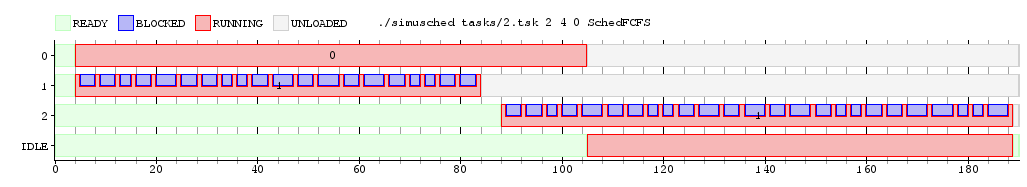
\includegraphics[width=\linewidth]{images/2_2nucleos.png}
    \label{fig:Task Consola}
    \caption{Rolando con 2 núcleos}
\end{figure}

En la Figura 3 se observa el diagrama de Gantt del mismo lote de tareas y scheduler de antes, pero esta vez bajo una CPU que cuenta con dos n\'ucleos. Al igual que el caso anterior, el \textit{switch\_cost} es de 4 ciclos, por lo que se demora esa cantidad de tiempo en empezar a correr las primeras tareas. A diferencia del caso anterior (en el que se contaba con un s\'olo n\'ucleo) tras este tiempo, pasan al estado \textit{runing} las primeras 2 tareas, TaskCPU y TaskConsola (de parametro \textit{$<$20, 2, 4$>$}), corriendo paralelamente (una en cada núcleo). De esta forma, la tarea TaskConsola en actual ejecuci\'on puede efectuar sus llamadas bloqueantes y mientras, la tarea TaskCPU continuar trabajando ininterrumpidamente. Tras finalizar la tarea identificada por el \textit{label} 1 del grafico (la TaskConsola 20 2 4), y el usual tiempo empleado para el cambio de contexto, el n\'ucleo asignado a dicha tarea pasa a otorgarle tiempo en el mismo a la \'ultima tarea restante. Mientras esta aún se mantiene corriendo, la tarea TaskCPU continua en estado \textit{runing}, y al finalizar pasa a asignarsele la tarea \textit{IDLE} al n\'ucleo previamente ocupado por TaskCPU; pues no le quedan mas tareas en el lote. La tarea TaskConsola (de parametro \textit{$<$25, 2, 4$>$}) efectua sus 25 llamadas bloqueantes y termina como siempre (en el FCFS), con un \textit{exit()} en su \'ultimo ciclo asignado.
\\
\\
A continuaci\'on se muestra en una tabla las latencias de cada tarea del \textit{lote2}. En el caso de las tareas de tipo TaskConsola, debido a que sus llamadas bloqueantes no duran un tiempo predeterminado, la latencia de la siguiente tarea es estimada entre un rango que resulta de asumir el mínimo y máximo tiempo que pueden durar bloquedas tras cada llamada.
\begin{table}[H]
\centering
\caption{Latencias}
\label{my-label}
\begin{tabular}{@{}lcc@{}}
\toprule
\multicolumn{1}{c}{Tarea} & 1 núcleo & 2 núcleos \\ \midrule
TaskCPU 100               & 4        & 4         \\
TaskConsola 20 2 4        & 109      & 4         \\
TaskConsola 25 2 4        & 174-214  & 69-109    \\ \bottomrule
\end{tabular}
\end{table}